\section{First Section}

\subsection{A Subsection}
	\begin{frame}{Introduction to Problem}{Spiral}
		\begin{itemize}
			\item Goal in SSL is, given $\{x_i,y_i\}_{i=1}^{M}$ and $\{x_i\}_{i=M+1}^{N}$, to predict $y_i(x_i)$ for $i=M+1, \dots , N$ where $M \ll N$.
		\end{itemize}
		\begin{figure}[H]
			\centering
			\hspace*{0cm}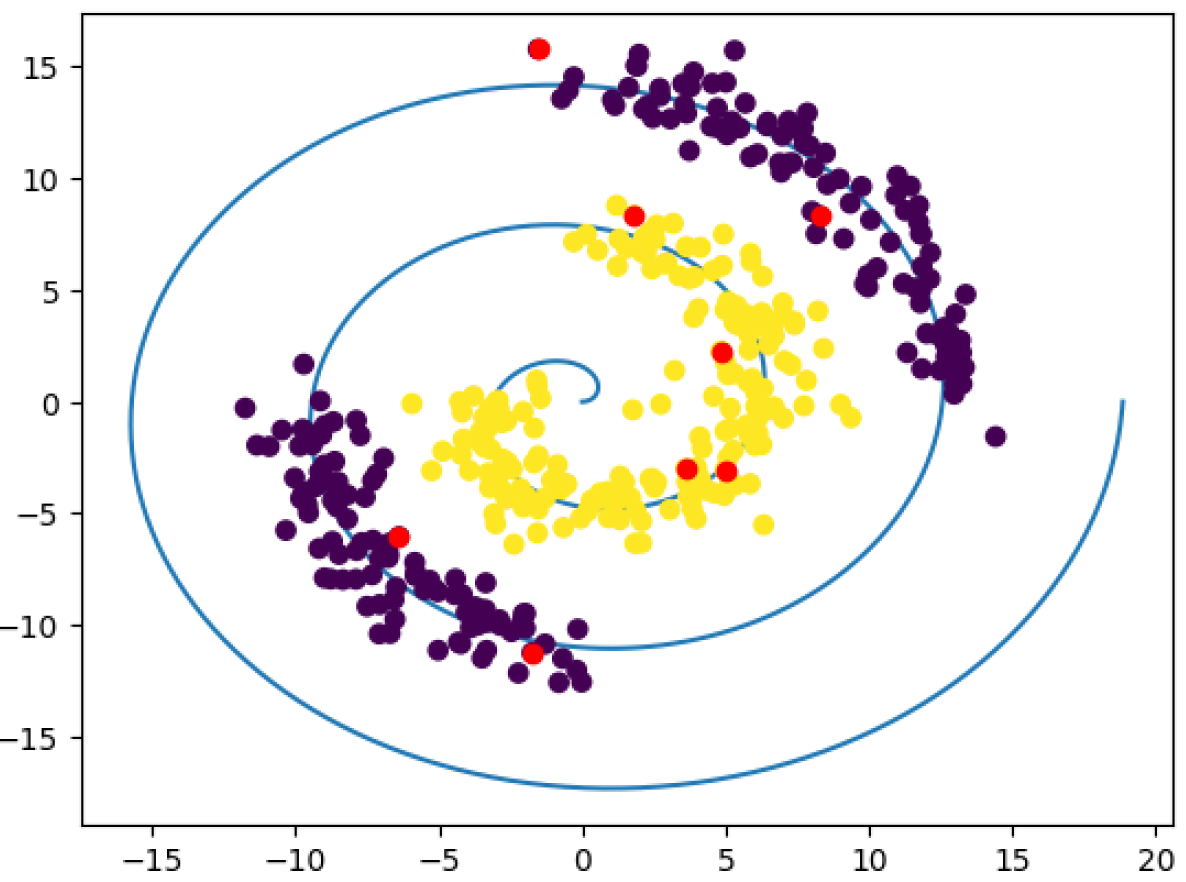
\includegraphics[width=0.75\textwidth,height=\textwidth,keepaspectratio]{/Users/Johnson/Documents/Amath_563/AMATH563_gssl/Complete Examples/Figs/SpiOg.png}
		\end{figure}
	\end{frame}

	\begin{frame}{GSSL}{Spiral}
		\begin{itemize}
			\item We leverage spectral geometric properties of the graph Laplacian matrix $L$.
			\item First, we construct our graphs by KNN or Proximity graph construction.
		\end{itemize}
		\begin{figure}[H]
			\centering
			\hspace*{0cm}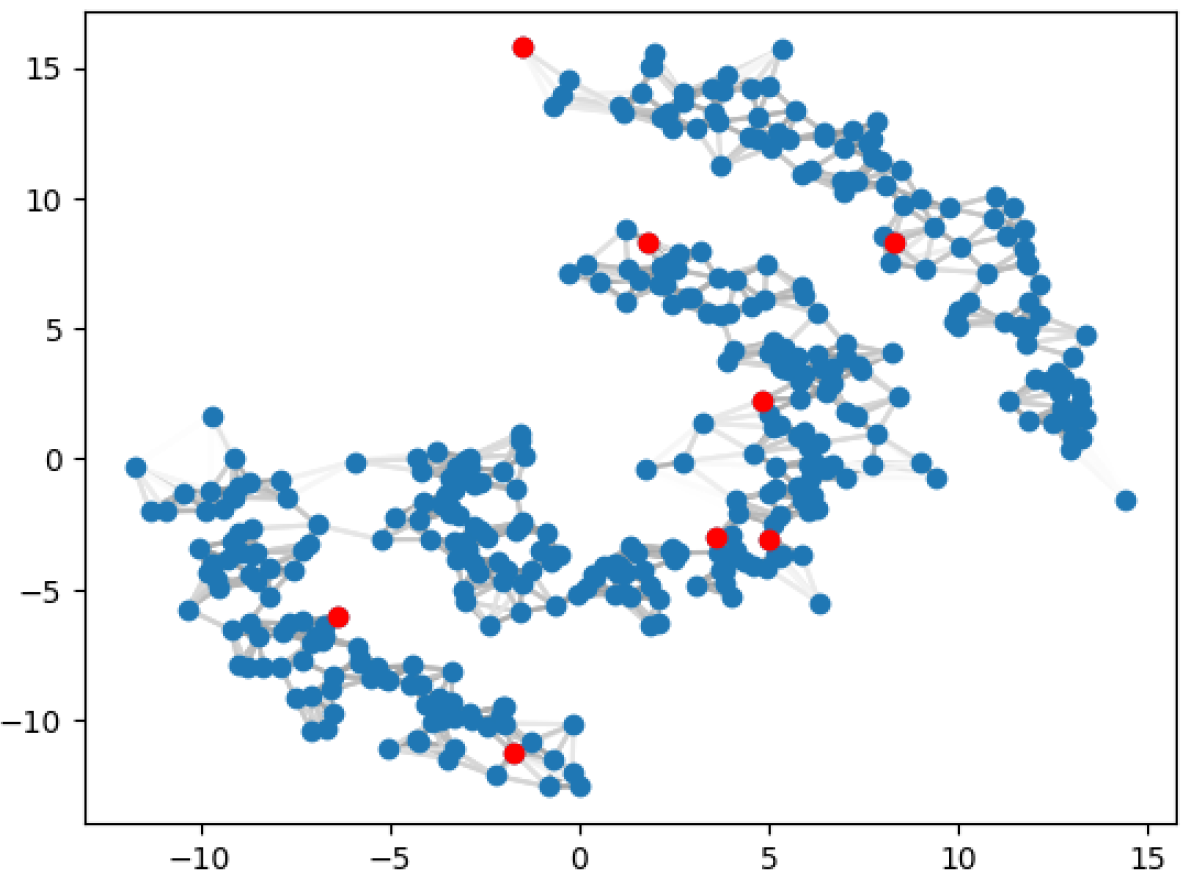
\includegraphics[width=0.6\textwidth,height=\textwidth,keepaspectratio]{/Users/Johnson/Documents/Amath_563/AMATH563_gssl/Complete Examples/Figs/SpiKNNRBF.png}
		\end{figure}
	\end{frame}

	\begin{frame}{Optimization Problem}{Setup and loss functions}
		\begin{itemize}
			\item General optimization
			\[\vec{f^*} = \argmin_{\vec{f} \in \R^{m}} \mathcal{L}(\vec{f};y) + \lambda \vec{f}^{T}C^{-1}\vec{f}\]
			where $\mathcal{L}$ is a loss function, either Probit or Regression loss in our case.
			\item Probit loss
			\[
				\mathcal{L}(\vec{f},y) = - \sum_{j=1}^{M}\log \Psi (\vec{f_j}y_j)	
			\]
			\item Regression loss
			\[
				\mathcal{L}(\vec{f},y) = \sum_{j=1}^{M}\paren{\vec{f}_{j} - y_{j}}^2
			\]
		\end{itemize}
	\end{frame}

	\begin{frame}{Optimization Problem}{Matérn kernel-regularization}
		\begin{itemize}
			\item General optimization
			\[\vec{f^*} = \argmin_{\vec{f} \in \R^{m}} \mathcal{L}(\vec{f};y) + \lambda \vec{f}^{T}C^{-1}\vec{f}\]
			where $C = (L + \tau^2 I)^{-\alpha}$, where $L$ is the graph Laplacian.
			\item In class, we showed $C$ is a kernel matrix. In fact, $C$ belongs to a class of kernels called the Matérn family that have the form
			\[
				K(x,y) = \kappa(\norm{x-y}), \kappa(t) = \frac{2^{1-\nu}}{\Gamma(\nu)}\paren{\sqrt{2\nu}\frac{t}{\gamma}}K_{\nu}\paren{\sqrt{2\nu}\frac{t}{\gamma}}	
			\]
			where $\Gamma$ is the Gamma function and $K_\nu$ is the modified Bessel function of the second kind.
			% TODO: why is this desriable? C is desriable bc it embeds the spectral geometric information that allows us to efficiently and successfuly create clusters! Remember that we are doing clustering and labelling at the same time; the label information in large part is coming from the spectral clustering we can perform on the connected components of the graph we create. C is literally how we embed the geometric information and how we actually leverage graphs.
		\end{itemize}
	\end{frame}